\documentclass[12pt]{ctexart}
\usepackage[dvipsnames,svgnames]{xcolor}
\usepackage{note}
\usepackage{longtable}
\usepackage{hyperref}
\usepackage{matlab}
\usepackage{amsmath} % 数学公式
\usepackage{amsthm} % 定理环境
\numberwithin{equation}{section} % 按 section 区分方程的编号
\newtheorem{theorem}{定理}[section] % 定义定理环境
% 格式和布局设置
% 使用multicol包来创建多列布局
% \usepackage{hyperref}
% \hypersetup{
%   colorlinks=true,
%   linkcolor=blue,
%   filecolor=magenta,      
%   urlcolor=blue,
%   pdftitle={Document with Links},
%   pdfpagemode=FullScreen,
% }
\usepackage{multicol}
\setlength{\columnsep}{0.1cm} % 设置列间距
\setlength{\columnseprule}{0.4pt} % 设置列间分界线
\usepackage[a4paper, margin=1in]{geometry} % 设置页面边距
\usepackage{indentfirst} % 首段缩进
\usepackage{setspace} % 行距设置
\usepackage{titlesec} % 标题格式设置
\usepackage{natbib} % 参考文献引用
\usepackage{fancyhdr} % 自定义页眉页脚
\usepackage{unicode-math} % Unicode 数学字体支持
% 设置数学字体
\setmathfont{Segoe UI Symbol}
% 定义正式文本框环境
\definecolor{formalshade}{rgb}{0.95,0.95,1} % 正式文本框颜色
\usepackage{framed}
\newenvironment{formal}{%
  \def\FrameCommand{%
    \hspace{2pt}%
    {\color{DarkBlue}\vrule width 2pt}%
    {\color{formalshade}\vrule width 4pt}%
    \colorbox{formalshade}%
  }%
  \MakeFramed{\advance\hsize-\width\FrameRestore}%
  \vspace{5pt}% 调整正式文本框上下的间距
}
{\endMakeFramed}
% 设置大标题格式
\titleformat{\section}
  {\bfseries\Large} % 标题字体加粗,设为大号
  {\thesection} % 标题编号
  {1em} % 标题与编号间距
  {} % 标题文本格式
% 设置小标题(subsection)格式
\titleformat{\subsection}
  {\bfseries\large} % 字体加粗,设为大号
  {\thesubsection} % 编号
  {1em} % 标题与编号间距
  {} % 标题文本格式

% 设置段落间距
\setlength{\parskip}{0.5\baselineskip} % 设为半个行高

% 设置行间距
\setstretch{1.2} % 行间距设置为1.2倍

% 设置标题之间的间距
\titlespacing*{\section}{0pt}{\baselineskip}{0.5\baselineskip} % 一级标题
\titlespacing*{\subsection}{0pt}{0.75\baselineskip}{0.25\baselineskip} % 二级标题


% 文档标题、作者、日期
\title{乌拉}
\author{李先宝}
\date{}

\begin{document}
\tableofcontents % 生成目录
\newpage
% \section{经济金融最优化问题}
% \subsection{}

\section{概率分布方法}
\subsection{经验分布函数}

根据\cite{司守奎}的$P_{184}$

一般地,设$x_1,x_2,\cdots,x_n$ 是总体$F$的一个容量为$n$ 的样本值。先将 $x_1,x_2,\cdots,x_n$ 按自

小到大的次序排列,并重新编号。设为
$$x_{(1)}\leq x_{(2)}\leq\cdots\leq x_{(n)}\:,$$

则经验分布函数$F_n(x)$的观察值
$$\begin{aligned}&\\&F_{n}(x)=\begin{cases}0,&\text{若 }x<x_{(1)}\:,\\\frac{k}{n},&\text{若 }x_{(k)}\leq x<x_{(k+1)}\:,\\\\1,&\text{若 }x\geqslant x_{(n)}\:.\end{cases}\\\end{aligned}$$
对于经验分布函数$F_n(x)$ ,格里汶科( Glivenko)在 1933 年证明了,当$n\to\infty$时$,F_n(x)$ 以概率 1 一致收敛于总体分布函数$F(x)$。因此,对于任一实数$x,当n$充分大时,经验分布函数的任一个观察值$F_n(x)$与总体分布函数 $F(x)$只有微小的差别,从而在实际上可当作 $F(x)$来使用。

\subsection{Q-Q图}
根据\cite{司守奎}的$P_{186}$

将经验分布函数的分位数点和分布模型的理论分位数点作为一对数组画在直角坐标图上,就是一个点,$n$个观测数据对应$n$个点,如果这$n$个点看起来像一条直线,说明观测数据与分布模型的拟合效果很好,以下简单地给出计算步骤。
判断观测数据$x_1,x_2,\cdots,x_n$是否来自于分布$F(x)$,画 Q-Q 图的步骤如下:
\begin{enumerate}
   

\item 将$x_1,x_2,\cdots,x_n$依大小顺序排列成:$x_{(1)}\leq x_{(2)}\leq\cdots\leq x_{(n)}$
\item 取$y_{i}= F^{- 1}($ ( $i- 1/ 2) / n$ $) , i= 1, 2, \cdots , n$。
\item  将$(y_i,x_{(i)}),i=1,2,\cdots,n$,这 $n$ 个点画在直角坐标图上。
\item 如果这$n$个点看起来呈一条 45°角的直线,从(0,0)到(1,1)分布,我们就相信
$x_{1},x_{2},\cdots,x_{n}$拟合分布$F(x)$的效果很好。
\end{enumerate}
\subsection{马尔可夫随机过程}
根据\cite{梅正阳}的$P_{125}$

马尔可夫过程是一类重要的随机过程或随机动态系统,具有如下特征: 
\begin{enumerate}
\item 系统在每个时刻所处的状态是随机的;
\item 系统从上一时刻的状态到下一时刻的状态按一定的概率转移;
\item 系统在下一时刻的状态只与当前时刻的状态和转移概率有关,与此前时刻的状态无关,即已知现在状态,将来的状态与过去无关(无后效性).
\end{enumerate}
\begin{mydef}{时间指标}
时间指标:系统按照时间顺序发展,连续和离散情形下的时间指标分别取
$t\in [ 0, + \infty )$ 或 $t= t_1, t_2, \cdots , t_k, \cdots$
\end{mydef}
\begin{mydef}{系统状态}
系统状态:在不同的时刻,系统呈现出的不同面貌称为状态.连续和离散情形下的状态分别表示为
$X(t)=x_i,X_t=x_t$ 的成 $X_n= x_n,X_n= x( t_n)$
\end{mydef}
马尔可夫性:
$$\Pr\{X(t_{n+1})=x_{n+1}\mid X(t_{1})=x_{1},X(t_{2})=x_{2},\cdots,X(t_{n})=x_{n}\}\\=\Pr\{X(t_{n+1})=x_{n+1}\mid X(t_{n})=x_{n}\},\quad t_{1}<t_{2}<\cdots<t_{n}<t_{n+1}$$
时间齐次性:状态转移概率与时间长度无关
 $$\Pr \{ X( t_{n+ 1}+ \tau ) \mid X( t_n+ \tau ) \}= Pr\left \{ X( t_{n+ 1}) \mid X( t_n) \right \}$$
一 步 状 态 转 移 概 率 : 系 统 从 $t_n$时刻的状态$i$转移到$t_m+1$时刻的状态$j$的概率, 记为
$$p_{ij}^{(n,n+1)}=\Pr\{X(t_{n+1})=j\mid X(t_n)=i\},n=0,1,2,...$$


多步状态转移概率:系统从$t_n$时刻的状态$i$转移到$t_n+m$时刻的状态$j$的概率,
记为
$$p_i^{(n,n+m)}=\Pr\{X(t_{n+m})=j\mid X(t_{n})=i\},m=0,1,2,...$$



简记为 $p_{ij}^{(m)}.$ 

状态转移概率矩阵:
$P= ( p_{ij}^{(n, n+ 1)}) = ( p_{ij})$, $P^{( m) }= ( p_{ij}^{( n, n+ m) }) = ( p_{ij}^{( m) })$
\begin{mytheo}{}
如果\( m > s \geqslant 0 \),则有 \( P_{ij}^{(n,n+m)} = \sum P_{ik}^{(n,n+s)} \cdot P_{kj}^{(n+s,n+m)} \)。
\end{mytheo}
由此推出$P^{(m)}=P^m$,得到多步状态转移方程

$$a(n+m)=P^m\bullet a(n)=P^{n+m}\bullet a(0)$$

其中$a(n)$为$t_n$时刻所有状态概率构成的向量.
\begin{myex}
    假设将人的健康状况分为健康和疾病两种状态,统计数据发现某地区某特定年龄段的人健康状态有如下规律:今年健康、明年仍保持健康状态的概率为 0.8;而今年患病、明年转为健康状态的概率为 0.7. 若保险公司要对该地区该年龄段投保人未来的健康状态作出估计,以制订保险金和理赔金的数额.问某人投保时健康,10 年后他仍处于健康状态的概率.
    \tcblower
    $\begin{aligned}
        \binom{a_{1}(n+1)}{a_{2}(n+1)} &= \begin{pmatrix} p_{11} & p_{21} \\ p_{12} & p_{22} \end{pmatrix} \binom{a_{1}(n)}{a_{2}(n)} \\
        &=\begin{pmatrix} 0.8 & 0.7 \\ 0.2 & 0.3 \end{pmatrix}\binom{a_{1}(n)}{a_{2}(n)} \\
        &= P^T \binom{a_{1}(n)}{a_{2}(n)}, \quad \text{其中 } P = \begin{pmatrix} 0.8 & 0.2 \\ 0.7 & 0.3 
        \end{pmatrix}\\
        &\text{初始状态向量的既可以是一固定的值,也可以为服从某一分布的随机向量}\end{aligned}$
    \end{myex}
    进一步分析:正则链与吸收链,以及首达概率,以及首返概率,见教材

    常用来解决
\begin{itemize}
  \item 存储问题
  \item 排队问题

  \item 网络流问题
\end{itemize}

\subsection{分布拟合检验}
根据\cite{夏爱生}的$P_{114}$
$\chi^2$检验法的基本思想如下:将随机试验可能结果的全体$\Omega$分为$k$个互不相容的事件$A_1,A_2,A_3,\ldots,A_k\left(\sum_{i=1}^kA_k=\Omega,A_iA_j=\phi,i\neq j,i,j=1,2,\ldots,k\right).$于是在假设$H_0$下, 我们可以计算$p_i=P(A_i)$ (或$\hat{p}_i=\hat{P}(A_i)),i=1,2,...,k.$在$n$次试验中,事件$A_i$出现的频率$f_i/n$ 与$p_i(\hat{p}_i)$ 往往有差异,但一般来说,若 $H_0$ 为真,且试验的次数又甚多时,则这种差异不应该很大.基于这种想法,皮尔逊使用统计量
$$\chi^2 = \sum_{i = 1}^k \frac{( f_i-np_i )^2}{np_i}\bigg( \text{或} \chi^2 = \sum_{i = 1}^k \frac{( f_i-n\hat{p}_i )^2}{n\hat{p}_i}\bigg)$$
$\chi^2$ 检验法:

$H_{0}:$总体 $x$ 的分布函数为$F(x)$,
$H_{1}:$总体 $x$ 的分布函数不是$F(x).$

构造统计量
$$\chi^2 = \sum_{i = 1}^k \frac{( f_i-np_i )^2}{np_i}\bigg( \text{或} \chi^2 = \sum_{i = 1}^k \frac{( f_i-n\hat{p}_i )^2}{n\hat{p}_i}\bigg)$$
\begin{mytheo}{分布拟合检验}
若$n$充分大,则当$H_0$为真时 (不论$H_0$中的分布属于什么分布),统计量 总是近似地服从自由度为$k-r-1$的$\chi^2$分布,其中$r$是被估计的参数的个数.
于是,若在假设$H_{0}$下算得式有
$$\chi^2\geqslant\chi_\alpha(k-r-1)$$
则在显著性水平$\alpha$下拒绝$H_0$,否则就接受.
注意:在使用$\chi^2$检验法时,要求样本容量$n$不小于 50,以及每个$np_i$都不小于 5,而
且$np_i$ 最好是在 5 以上.否则应适当地合并 $A_i$,以满足这个要求.
\end{mytheo}
\begin{lstlisting}{分布拟合检验}
  clc
x= [141 148 132 138 154 142 150 146 155 158...
150 140 147 148 144 150 149 145 149 158...
143 141 144 144 126 140 144 142 141 140...
145 135 147 146 141 136 140 146 142 137...
148 154 137 139 143 140 131 143 141 149...
148 135 148 152 143 144 141 143 147 146...
150 132 142 142 143 153 149 146 149 138...
142 149 142 137 134 144 146 147 140 142...
140 137 152 145];
mm= minmax(x) %求数据中的最小数和最大数
hist(x,8) %画直方图
fi= [length(find(x< 135)),...
length(find(x> = 135&x< 138)),...
length(find(x> = 138&x< 142)),...
length(find(x> = 142&x< 146)),...
length(find(x> = 146&x< 150)),...
length(find(x> = 150&x< 154)),...
length(find(x> = 154))] %各区间上出现的频数
mu= mean(x),sigma= std(x) %均值和标准差
fendian= [135,138,142,146,150,154] %区间的分点
p0= normcdf(fendian,mu,sigma) %分点处分布函数的值
p1= diff(p0) %中间各区间的概率
p= [p0(1),p1,1- p0(6)] %所有区间的概率
chi= (fi- 84* p).^2./(84* p)
chisum= sum(chi) %皮尔逊统计量的值
x_a= chi2inv(0.9,4) %chi2 分布的 0.9 分位数
\end{lstlisting}
\subsection{足球门踢球问题}
根据\cite{韩中庚}$P_{116}$
\begin{myex}
  在足球比赛中,球员在对方球门前不同的位置起脚射门对球门的威胁是不一样的.在球门的正前方的威胁要大于在球门两侧射门;近距离的射门对球门的威胁要大于远射.已知标准球场长为 104 m,宽为 69 m;球门高为 2.44 m,宽为$7.32m.$
实际中,球员之间的基本素质可能有一定差异,但对于职业球员来讲一般可认为这种差别不大.另外,根据统计资料显示,射门时球的速度一般在 10 m/s 左右.请你结合球场和足球赛的实际情况建模分析,并研究下列问题:
\begin{enumerate}
\item 针对球员在不同位置射门对球门的威胁度进行研究,并绘制出球门的
危险区域;
\item 在有一名守门员防守的情况下,对球员射门的威胁度和危险区域作进
一步的研究.
\end{enumerate}
% \tcblower

\end{myex}
问题的要点分析
\begin{itemize}
  \item 当球员相对球门的位置确定时,球飞向球门的落点具有随机性,应该满足一个二维正态分布。
  \item 其中不同位置的优劣可以通过方差来反映。
  \item 所以我们可以建立二维坐标系,对球门进行积分就可以得到命中概率,并把该命中概率定义为威胁程度。注意这个球门的积分可以下来进行操作一下。
  \item 时间 $t$ 为球从射门到进入球门的时间,对于守门员的捕获概率 $p_{0}(t,y,z)$,当 $t$ 一定时,概率以守门员为中心向周围衰减的二维函数。当 $t$ 变小时,整个曲线的峰度增大;当 $t$ 变大时,整个曲线的峰度减小;当 $t$ 趋于无穷大时,整个曲线的峰度增大。所以可以得到形式 $p_{0}(t,y,z) = \mathrm{e}^{-\frac{(y-a)^{2}+(z-1.25)^{2}}{ct}}$。
  \item 在问题(1)的基础上,对球员在球场上一点 $A(x_{0},y_{0})$ 射人球门的概率应修正如下:
  $$ p_{D}(x_{0},y_{0};y_{1},z_{1}) = \iint_{D} f(y,z) [1 - p_{0}(t,y,z)] \, \mathrm{d}y \, \mathrm{d}z $$
\end{itemize}
\section{相关系数分析}
\subsection{正态分布检验}
根据\cite{清风}第五讲

一般我们需要检验数据是否来自一个正态总体
\subsubsection{正态分布JB检验(大样本 n>30)}
雅克-贝拉检验(Jarque-Bera test)
$$JB\:=\:\dfrac{n}{6}[S^2+\dfrac{(K-3)^2}{4}]$$

对于一个随机变量 $\{X_i\}$ ,假设其偏度为$S$,峰度为$K$,那么我们可以构造$JB$统计量:
可以证明,如果 $\{X_i\}$ 是正态分布,那么在大样本情况下$JB\sim \chi ^2( 2)$ (自由度为2的卡方分布)

注:正态分布的偏度为0,峰度为3


那么进行假设检验的步骤如下:

$H_0{: \text{该 随 机 变 量 服 从 正 态 分 布 }}$ $H_1{: \text{该 随 机 变 量 不 服 从 正 态 分 布 }}$
然后计算该变量的偏度和峰度,得到检验值$JB^*$,并计算出其对应的$p$值将$p$值与0.05比较,如果小于0.05则可拒绝原假设,否则我们不能拒绝原假设。
\begin{lstlisting}{JB检验}
  x = normrnd ( 2, 3, 100, 1) ; 
% 生成100*1的随机向量,每个元素是均值为2,标准差为3的正态分布
skewness(x) %偏度
kurtosis(x) %峰度
%%正态分布检验
%检验第一列数据是否为正态分布
[h,p]=jbtest(Test(:,1),0.05)
%[h,p]=jbtest(x,alpha)alpha为显著性水平,默认为0.05
%h=0,则接受原假设,即数据服从正态分布
% 用循环检验所有列的数据
n_c = size(Test,2); % number of column 数据的列数
H=zeros(1,6)
P=zeros(1,6)
for i = 1:n_c
[h, p]=jbtest(Test(:,i),0.05);
H(i)=h;
P(i)=p;
end
disp(H)
disp(P)
\end{lstlisting}
\subsubsection{小样本: Shapiro-wilk检验}
对于小样本$3\leqslant n\leqslant50$
采用
$Shapiro-wilk$夏皮洛-威尔克检验

$H_0$:该随机变量服从正态分布$H_1$:该随机变量不服从正态分布
计算出威尔克统计量后,得到相应的$p$ 值
将$p$值与0.05比较,如果小于0.05则可拒绝原假设,否则我们不能拒绝原假设。

具体操作见清风教学文档的第五讲里SPSS操作
\subsection{Pearson相关系数及其检验}
\begin{mydef}{Pearson相关系数}
  

样本Pearson 相关系数:$$r_{XY}=\frac{\mathrm{Cov}(X,Y)}{S_XS_Y}$$
\end{mydef}
皮尔逊相关系数假设检验的条件

第一,实验数据通常假设是成对的来自于正态分布的总体。因为我们在求皮尔逊相关性系数以后,通常还会用t检验之类的方法来进行皮尔逊相关性系数检验,而t检验是基于数据呈正态分布的假设的。

第二,实验数据之间的差距不能太大。皮尔逊相关性系数受异常值的影响比较大。

第三:每组样本之间是独立抽样的。构造t统计量时需要用到。


p值判断法

$\text{对于皮尔逊相关系数}r\text{而言,在满足一定条件下,我们可以构造统计量:}\\t = r\sqrt{\frac{n-2}{1-r^{2}}} , \text{可以证明}t\text{是服从自由度为}n \text{-2的}t \text{分布}$

我们得到的检验值$t^*$,根据这个值,我们可以计算出其对应的那个概率$p$

$p$值>0.01,说明在99\%的置信水平无法拒绝原假设; 

$p>0.05$,说明在95\%的置信水平上无法拒绝原假设;

 $p>0.10$,说明在90\%的置信水平上无法拒绝原假设;

$p<0.01$,说明在99\%的置信水平上拒绝原假设;

 $p<0.05$,说明在95\%的置信水平上拒绝原假设;

 $p<0.10$,说明在90\%的置信水平上拒绝原假设;

\begin{lstlisting}{p值判断法}
  %%计算各列之间的相关系数以及p值
[ R, P ] = corrcoef(Test)
\end{lstlisting}
\subsection{斯皮尔曼spearman相关系数及其检验}

\begin{mydef}{斯皮尔曼spearman相关系数}
定义:$X$和$Y$为两组数据,其斯皮尔曼(等级)相关系数:
$$r_{s}=1-\frac{6\sum_{i=1}^{n}d_{i}^{2}}{n\left(n^{2}-1\right)}$$
其中,$d_i$为$X_i$和$Y_i$之间的等级差。
(一个数的等级,就是将它所在的一列数按照从小到大排序后,这个数所在的位置)
可以证明:$r_s$位于-1和1之间。
\end{mydef}


\begin{lstlisting}{spearman相关系数的代码示例}
  %% MATLAB求解皮尔逊相关系数
RX = [2 5 3 4 1]
RY = [1 4.5 3 4.5 2]
R = corrcoef(RX,RY)
X = [3 8 4 7 2]' % 一定要是列向量哦,一撇'表示求转置
Y = [5 10 9 10 6]'
coeff = corr(X , Y , 'type' , 'Spearman')
\end{lstlisting}

假设检验分为小样本和大样本
分为小样本和大样本两种情况:

小样本情况,即$n\leq30$时,直接查临界值表即可。

大样本情况下,统计量$r_s\sqrt{n-1}$~$N(0,1)$
$$H_0:r_s=0,\:H_1:r_s\neq0$$
我们计算检验值$r_s\sqrt{n-1}$,并求出对应的$p$ 值与0.05相比即可。
\begin{lstlisting}{大样本检验}
  % 直接给出相关系数和p值
[R,P]=corr(Test, 'type' , 'Spearman')
\end{lstlisting}
\subsection{两种相关系数的比较}


斯皮尔曼相关系数和皮尔逊相关系数选择:
\begin{enumerate}
\item 连续数据,正态分布,线性关系,用pearson相关系数是最恰当,当然用
spearman相关系数也可以,就是效率没有pearson相关系数高。
\item 上述任一条件不满足,就用spearman相关系数,不能用pearson相关系数。
\item 两个定序数据之间也用spearman相关系数,不能用pearson相关系数。
定序数据是指仅仅反映观测对象等级、顺序关系的数据,是由定序尺度计量
形成的,表现为类别,可以进行排序,属于品质数据。
例如:优、良、差;
我们可以用1表示差、2表示良、3表示优,但请注意,用2除以1得出的2并不代表任何含义。定序数据最重要的意义代表了一组数据中的某种逻辑顺序。
注:斯皮尔曼相关系数的适用条件比皮尔逊相关系数要广,只要数据满足单调关系(例如线性函数、指数函数、对数函数等)就能够使用。
\end{enumerate}
\section{综合评价与决策方法}
\subsection{TOPSIS算法即理想解法}
根据\cite{司守奎}$Page_{411}$
TOPSIS 法的具体算法步骤如下:
\begin{enumerate}
\item 用向量规划化的方法求得规范决策矩阵。设多属性决策问题的决策矩阵
$A=(a_{ij})_{m\times n}$(可以理解成$m$个对象$n$个指标),规范化决策矩阵 $B=(b_{ij})_m\times n$(常用标准化处理,常要考虑指标的类型如效用型、成本型或区间型)
其中
$$b_{ij}=a_{ij}\Big/\sqrt{\sum_{i=1}^{m}a_{ij}^{2}}\:,\:i=1\:,2\:,\cdots,m\:;\:j=1\:,2\:,\cdots,n.$$

\item 构造加权规范阵$C=(c_{ij})_{m\mathrm{x}n}$。设由决策人给定各属性的权重向量(一般可以考虑熵权法,但是也不是完全的合理,最好还是看看层次分析法里面的权重确定的方法)为$w=[w_1$,
$w_{2},\cdots,w_{n}]^{\mathrm{T}}$,则

$$c_{ij}=w_{j}\:\cdot\:b_{ij}\:,i=1\:,2\:,\cdots,m\:;\:j=1\:,2\:,\cdots,n.$$
\item 确定正理想解$C^{*}$和负理想解$C^{0}$。设正理想解$C^{*}$的第$j$个属性值为$c_j^{*}$,负理想
解 $C^{0}$ 第$j$ 个属性值为 $c_j^0$,则
$$\text{正理想解}:c_j^*=\begin{cases}\max_ic_{ij},j\text{ 为效益型属性,}\\\min_ic_{ij},j\text{ 为成本型属性,}\end{cases}j=1,2,\cdots,n,$$
负理想解:$c_j^0= \begin{cases} \min _ic_{ij}, j\text{ 为 效 益 型 属 性 , }\\ \max c_{ij}\text{ 为 成 本 型 属 性 }. & \end{cases} j= 1, 2, \cdots , n.$ (14.4)
\item 计算各方案到正理想解与负理想解的距离。备选方案$d_i$到正理想解的距离为
$$s_{i}^{*}\:=\:\sqrt{\sum_{j=1}^{n}\:(\:c_{ij}\:-\:c_{j}^{*}\:)^{2}}\:,i=1\:,2\:,\cdots,m\:;$$
备选方案$d_i$到负理想解的距离为
$$s_{i}^{0}\:=\:\sqrt{\sum_{j=1}^{n}\:(\:c_{ij}\:-\:c_{j}^{0}\:)^{2}}\:,i\:=\:1\:,2\:,\cdots,m.$$
\item 计算各方案的排序指标值(即综合评价指数),即
$$f_{i}^{*}=s_{i}^{0}/(\:s_{i}^{0}+s_{i}^{*}\:)\:,i=1\:,2\:,\cdots,m.$$
\item 按$f_i^*$由大到小排列方案的优劣次序。
\end{enumerate}
\subsection{灰色关联分析}
根据\cite{司守奎}$Page_{424}$
灰色关联度分析具体步骤如下:
\begin{enumerate}

\item 确定比较数列和参考数列。设评价对象有$m$个,评价指标变量有$n$个,每个指
标变量 $x_j(j=1,2,\cdots,n)$都是效益型指标变量。比较数列为
$$a_{i}=\{\:a_{i}(j)\:|\:j\:=\:1\:,2\:,\cdots,n\}\:,i\:=\:1\:,2\:,\cdots,m\:,$$
式中:$a_i(j)$是第$i$个 评 价 对 象 关 于 第 $j$个指标变量$x_j$的取值。
参考数列为$a_0=\{a_0(j)\mid j=1,2,\cdots,n\}$ ,一般取$a_0(j)=\max_{1\leq i\leq m}\{a_i(j)\}$ ,即参考数列相当
于一个虚拟的最好评价对象的各指标值。
\item 确定各指标对应的权重。可用层次分析法等确定各指标对应的权重$w=[w_1$,
$w_{2},\cdots,w_{n}]$,其中$w_j,j=1,2,\cdots,n$为第$j$个评价指标对应的权重。
\item 计算灰色关联系数:
$$\xi_{i}(j)=\frac{\min_{1\leq s\leq m}\min_{1\leq s\leq m}\mid a_{0}(t)-a_{s}(t)\mid+\rho\max_{1\leq s\leq m}\max_{1\leq s\leq m}\mid a_{0}(t)-a_{s}(t)\mid}{\mid a_{0}(j)-a_{i}(j)\mid+\rho\max_{1\leq s\leq m}\max_{1\leq s\leq m}\mid a_{0}(t)-a_{s}(t)\mid},i=1,2,\cdots,m,j=1,2,\cdots,n.$$
$\xi_i(j)$为比较数列$a_i$对参考数列$a_0$在 第 $j$个指标上的关联系数,其中$\rho\in[0,1]$为分辨系数。其中,$\min_{1\leq s\leq m}\min_{1\leq t\leq n}|a_0(t)-a_s(t)|_{\mathrm{、}\operatorname*{\max}_{1\leq s\leq m}1\leq i\leq n}|a_0(t)-a_s(t)|$分别称为两级最小差及两级最大差
一般来讲,分辨系数$\rho$越大,分辨率越大;$\rho$越小,分辨率越小。
\item 计算灰色加权关联度。灰色加权关联度的计算公式为
$$r_{i}=\sum_{k=1}^{n}w_{k}\xi_{i}(\:k\:)\:,$$
式中:$r_\mathrm{i}$为第$i$个评价对象对理想对象的灰色加权关联度,若没有给出各指标变量的权
重,则各指标变量取相等的权重,即$w_j=1/n,j=1,2,\cdots,n$。
\item 评价分析。根据灰色加权关联度的大小,对各评价对象进行排序,可建立评价对
象的关联序,关联度越大,其评价结果越好。所以本质还是求关联度的问题,只是我们得到与最优虚拟对象关联度最好就是评价效果最好的嘛。

\end{enumerate}
\section{聚类分析}
根据\cite{司守奎}$Page_{262}$
聚类分析又称群分析,是对多个样本( 或指标)进行定量分类的一种多元统计分析方
法。对样本进行分类称为 Q 型聚类分析,对指标进行分类称为 R 型聚类分析。
\subsection{Q型聚类}
\subsubsection{类的相似性度量}

如果有两个样本类 $G_1$和$G_2$可以用下面的一系列方法度量它们之间的距离(即相似性)。

离差平方和法( Sum of Squares Method)
 若记$$D_{1}=\sum_{x_{i}\in G_{1}}(x_{i}-\overline{x}_{1})^{\mathrm{T}}(x_{i}-\overline{x}_{1})\:,D_{2}=\sum_{x_{j}\in G_{2}}(x_{j}-\overline{x}_{2})^{\mathrm{T}}(x_{j}-\overline{x}_{2})\:,\\D_{12}=\sum_{x_{k}\in G_{1}\cup G_{2}}(x_{k}-\overline{x})^{\mathrm{T}}(x_{k}-\overline{x})\:,$$
式中
$$\overline{x}_{1}=\frac{1}{n_{1}}\sum_{x_{i}\in G_{1}}x_{i}\:,\overline{x}_{2}=\frac{1}{n_{2}x_{j}\in G_{2}}x_{j},\overline{x}=\frac{1}{n_{1}\:+\:n_{2}x_{k}\in G_{1}\cup G_{2}}x_{k}\:,$$
则定
$$D(\:G_{1}\:,G_{2}\:)=D_{12}-D_{1}-D_{2}.$$
事实上,若$G_1,G_2$ 内部点与点距离很小,则它们能很好地各自聚为一类,并且这两类又能

够充分分离(即$D_{12}$很大),这时必然有$D=D_{12}-D_{1}-D_{2}$很大。因此,按定义可以认为,两类$G_{_1},G_{_2}$之间的距离很大。离差平方和法最初是由 Ward 在 1936 年提出,又称Ward法
  
\subsubsection{聚类图}
\begin{enumerate}


  \item 计 算  $n$个 样 本 点 两 两 之 间 的 距 离 $\left | d_{ij}\right | $,记为矩阵$D=(d_ij)_nx_n\circ$
  \item 首先构造$n$个类,每一个类中只包含一个样本点,每一类的平台高度均为0。
  \item 合并距离最近的两类为新类,并且以这两类间的距离值作为聚类图中的平台
高度。
\item 计算新类与当前各类的距离,若类的个数已经等于 1,转人步骤(5),否则回到步

骤(3)。

\item 画聚类图。

\item  决定类的个数和类。
\end{enumerate}
\subsubsection{matlab聚类分析相关命令}
\begin{enumerate}
  \item pdist

  $Y=pdist(X)$计算$m\times p$矩阵 X(看作$m$个$p$维行向量)中两两行对象间的欧几里得距离。对于有$m$个对象组成的数据集,共有$(m-1)\cdot m/2$个两两对象组合。
  
  输出 Y 是包含距离信息的长度为( $m-1)\cdot m/2$的向量。可用 squareform 函数将此向量转换为方阵,这样可使矩阵中的元素(i,j)对应原始数据集中对象i和¡间的距离。
\item zscore

对数据矩阵进行标准化处理,处理方式为
$$\widetilde{x}_{ij}=\frac{x_{ij}-\overline{x}_{j}}{s_{j}},$$
式中:$\bar{x}_j,s_j$ 为矩阵 $X=(x_{ij})_m\mathrm{x}_n$每一列的均值和标准差。

\end{enumerate}
\subsection{R型聚类}
\subsubsection{变量的相似性度量}


在对变量进行聚类分析时,首先要确定变量的相似性度量,常用的变量相似性度量有
两种。
\begin{enumerate}
\item 相关系数。记变量$x_j$的取值$[x_{ij},x_{2i},\cdots,x_{mj}]^{\mathrm{T}}\in\mathbf{R}^{m}(j=1,2,\cdots,p)$。则可以用两

变量$x_j$与$x_k$的样本相关系数作为它们的相似性度量,即

$$r_{jk}=\frac{\sum_{i=1}^{m}\left(x_{ij}-\overline{x}_{j}\right)\left(x_{ik}-\overline{x}_{k}\right)}{\left[\sum_{i=1}^{m}\left(x_{ij}-\overline{x}_{j}\right)^{2}\sum_{i=1}^{m}\left(x_{ik}-\overline{x}_{k}\right)^{2}\right]^{\frac{1}{2}}},\:j,k=1,2,\cdots,p,$$
式中:$\bar{x}_j=\frac1m\sum_{i=1}^mx_{ij}\circ$

在对变量进行聚类分析时,利用相关系数矩阵 R=($r_ij)_{p\times p}$是最多的。
\item  夹角余弦。也可以直接利用两变量$x_j$与$x_k$的夹角余弦$r_{jk}$来定义它们的相似性
度量,有

$$r_{jk}=\frac{\sum_{i=1}^{m}x_{ij}x_{ik}}{\left(\sum_{i=1}^{m}x_{ij}^{2}\sum_{i=1}^{m}x_{ik}^{2}\right)^{\frac{1}{2}}},\:j,k=1,2,\cdots,p.$$
各种定义的相似度量均应具有以下两个性质:
1. 对于一切 \( j, k \),\(|r_{ik}| \leq 1\)。
2. 对于一切 \( j, k \),\( r_{jk} = r_{kj} \)。

\(|r_{jk}|\) 越接近 1,\( x_i \) 与 \( x_k \) 越相关或越相似。 \(|r_{jk}|\) 越接近 0,\( x_i \) 与 \( x_k \) 的相似性越弱。
\end{enumerate}
\subsubsection{变量聚类法}

类似于样本集合聚类分析中最常用的最短距离法、最长距离法等,变量聚类法采用了与系统聚类法相同的思路和过程。在变量聚类问题中,常用的有最长距离法、最短距离法等。
\section{主成分分析(PCA)}
\subsection{基本思想}
根据\cite{清风}第十四讲的内容
\begin{equation}
\begin{gathered}
  \text{假设有} n \text{ 个样本,} p \text{ 个指标,则可构成大小为} n \times p \text{ 的样本矩阵} x \text{:} \\
  x = 
  \begin{bmatrix}
  x_{11} & x_{12} & \cdots & x_{1p} \\
  x_{21} & x_{22} & \cdots & x_{2p} \\
  \vdots & \vdots & \ddots & \vdots \\
  x_{n1} & x_{n2} & \cdots & x_{np}
  \end{bmatrix}
  = (x_1, x_2, \ldots, x_p) \\
  \text{假设我们想找到新的一组变量} z_1, z_2, \ldots, z_m (m \leq p), \text{ 且它们满足:} \\
  \left\{
  \begin{array}{l}
  z_1 = l_{11}x_1 + l_{12}x_2 + \cdots + l_{1p}x_p \\
  z_2 = l_{21}x_1 + l_{22}x_2 + \cdots + l_{2p}x_p \\
  \vdots \\
  z_m = l_{m1}x_1 + l_{m2}x_2 + \cdots + l_{mp}x_p
  \end{array}
  \right.
  \end{gathered}
\end{equation}

系数$l_{ij}$的确定原则:

$(1)z_{i}$与$z_j(i\neq j;i,j=1,2,\cdotp\cdotp\cdotp,m)$相互无关;

$(2)z_1$是$x_1,x_2,\cdots,x_p$的一切线性组合中方差最大者;

$(2)z_2$是与$z_1$不相关的$x_1,x_2,\cdotp\cdotp\cdotp,x_p$的所有线性组合中方差最大者;

(3)依次类推,$z_m$是与$z_1,z_2,\cdotp\cdotp\cdotp,z_{m-1}$不相关的$x_1,x_2,\cdotp\cdotp\cdotp,x_p$的所有线性
组合中方差最大者。

(4)新变量指标$z_1,z_2,\cdotp\cdotp\cdotp,z_m$分别称为原变量指标$x_1,x_2,\cdotp\cdotp\cdotp,x_p$的第一,
第二,...,第$m$主成分。                 

\subsection{PCA的计算步骤}
根据\cite{司守奎}$Page_{282}$
计算步骤如下
\begin{enumerate}
  \item 对原始数据进行标准化处理。假设进行主成分分析的指标变量有 $m$ 个,分别为$x_1,x_2,\cdotp\cdotp\cdotp,x_m$,共有$n$个评价对象,第$i$个评价对象的第$j$个指标的取值为$a_{ij}$。将各指标值$a_{ij}$转换成标准化指标值 $\widetilde{a}_{ij}$,有
  $$\widetilde{a}_{ij}=\frac{a_{ij}-\mu_{j}}{s_{j}},\:i=1\:,2\:,\cdots,n\:;\:j=1\:,2\:,\cdots,m\:,$$
  式中:$\mu_j=\frac1n\sum_{i=1}^{n}a_{ij};s_{j}=\sqrt{\frac1{n-1}\sum_{i=1}^{n}\left(a_{ij}-\mu_{j}\right)^{2}},j=1,2,\cdots,m$,即$\mu_j,s_{j}$ 为第$j$ 个指标的样本
  均值和样本标准差。
  
  对应地,称
  $$\widetilde{x_{j}}=\frac{x_{j}-\mu_{j}}{s_{j}},\:j=1,2,\cdots,m\:,$$
  为标准化指标变量。
  \item $\text{ 计算相关系数矩阵 }R\text{。相关系数矩阵 }R=\left(r_{ij}\right)_{m\times m},\text{有}\\r_{ij}=\frac{\sum_{k=1}^{n}\widetilde{a}_{ki}\cdot\widetilde{a}_{kj}}{n-1},i,j=1,2,\cdots,m,\\\text{式中:}r_{ii}=1,r_{ij}=r_{ji},r_{ij}\text{为第 }i\text{ 个指标与第 }j\text{ 个指标的相关系数。}$
  \item 计算特征值和特征向量。计算相关系数矩阵$R$的特征值$\lambda_1\geq\lambda_2\geq\cdots\geq\lambda_m\geq0$, 及对应的特征向量$u_1,u_2,\cdots,u_m$,其中$u_j=[u_{ij},u_{2j},\cdots,u_{mj}]^\mathrm{T}$,由特征向量组成 $m$ 个新的指标变量:
  \[
\begin{aligned}
y_{1} &= u_{11}\widetilde{x}_{1} + u_{21}\widetilde{x}_{2} + \cdots + u_{m1}\widetilde{x}_{m} \\
y_{2} &= u_{12}\widetilde{x}_{1} + u_{22}\widetilde{x}_{2} + \cdots + u_{m2}\widetilde{x}_{m} \\
\vdots \\
y_{m} &= u_{1m}\widetilde{x}_{1} + u_{2m}\widetilde{x}_{2} + \cdots + u_{mm}\widetilde{x}_{m}
\end{aligned}
\]
  式中:$y_1$为第 1 主成分;$y_2$为第 2 主成分,.........;$y_m$为第$m$主成分。
  \item 选择 $p(p\leq m)$个主成分,计算综合评价值。
  计算特征值$\lambda_j(j=1,2,\cdots,m)$的信息贡献率和累积贡献率。称
  $$b_{j}=\frac{\lambda_{j}}{\sum_{k=1}^{m}\lambda_{k}},j=1,2,\cdots,m$$
  为主成分$y_j$的信息贡献率,同时,有
  
  
  $$\alpha_p=\frac{\sum_{k=1}^p\lambda_k}{\sum_{k=1}^m\lambda_k}$$
  为 主 成 分 $y _1, y  _2, \cdotp \cdotp \cdotp \cdotp , y  _p$ 的 累 积 贡 献 率 。当 $\alpha _p$ 接 近 于 1(一 般 取 $\alpha _p= 0. 85, 0. 90, 0. 95)$时 , 则选择前$p$个指标变量$y_1,y_2,\cdotp\cdotp\cdotp,y_p$作为$p$个主成分,代替原来$m$个指标变量,从而可对$p$个主成分进行综合分析。
\end{enumerate}
\subsection{主成分的说明及应用}
根据\cite{清风}第十四讲的内容
\begin{enumerate}
  \item 主成分分析是一种降维方法实际运用有以下说明
\begin{itemize}
  \item 在主成分分析中。我们首先应保证所提取的前几个主成分的累计贡献率达到一个较高的水平,其次对这些被提取的主成分必须都能够给出符合实际背景和意义的解释。
  \item 主成分的解释其含义一般多少带有点模糊性,不像原始变量的含义
  那么清楚、确切,这是变量降维过程中不得不付出的代价。因此,提取的主成分个数m通常应明显小于原始变量个数p(除非p本身较小),否则维数降低的“利”可能抵不过主成分含义不如原始变量清楚的“弊”。
  \item 如果原始变量之间具有较高的相关性,则前面少数几个主成分的累
  计贡献率通常就能达到一个较高水平,也就是说,此时的累计贡献率通
  常较易得到满足。
  \item 主成分分析的困难之处主要在于要能够给出主成分的较好解释,所提取的主成分中如有一个主成分解释不了,整个主成分分析也就失败了。
  \item 主成分分析是变量降维的一种重要、常用的方法,简单的说,该方
  法要应用得成功。一是靠原始变量的合理洗取。二是靠“运气”。
\end{itemize}


\item 应用具有以下几个方面:
\begin{itemize}
  \item 主成分回归可用来解决多重共线性的问题
  \item 用以主成分聚类,其最大的意义就是能帮我们可视化最后的聚类效果,
\end{itemize}
\end{enumerate}

\section{因子分析}

\subsection{因子分析和主成分分析的对比}
\begin{equation*}
  \begin{aligned}
  &\text{假设有} n \text{ 个样本,} p \text{ 个指标,则可构成大小为 } n \times p \text{ 的样本矩阵 } x = \\
  &\begin{bmatrix}
  x_{11} & x_{12} & \cdots & x_{1p} \\
  x_{21} & x_{22} & \cdots & x_{2p} \\
  \vdots & \vdots & \ddots & \vdots \\
  x_{n1} & x_{n2} & \cdots & x_{np}
  \end{bmatrix}
  = (x_1, x_2, \cdots, x_p) \\
  &\text{主成分分析:} \\
  &x_1, x_2, \cdots, x_p \Rightarrow z_1, z_2, \cdots, z_m (m \leq p), \text{ 且它们满足:} \\
  &\left\{
  \begin{array}{l}
  z_1 = l_{11}x_1 + l_{12}x_2 + \cdots + l_{1p}x_p \\
  z_2 = l_{21}x_1 + l_{22}x_2 + \cdots + l_{2p}x_p \\
  \vdots \\
  z_m = l_{m1}x_1 + l_{m2}x_2 + \cdots + l_{mp}x_p
  \end{array}
  \right. \\
  &z_1, z_2, \cdots, z_m \text{ 是 } m \text{ 个主成分,可以看出,主成分实际上就是各指标的线性组合。} \\
  &\text{因子分析:} \\
  &x_1, x_2, \cdots, x_p \Rightarrow f_1, f_2, \cdots, f_m (m \leq p), \text{ 且它们满足:} \\
  &\left\{
  \begin{array}{l}
  x_1 = u_1 + a_{11}f_1 + a_{12}f_2 + \cdots + a_{1m}f_m + \varepsilon_1 \\
  x_2 = u_2 + a_{21}f_1 + a_{22}f_2 + \cdots + a_{2m}f_m + \varepsilon_2 \\
  \vdots \\
  x_p = u_p + a_{p1}f_1 + a_{p2}f_2 + \cdots + a_{pm}f_m + \varepsilon_p
  \end{array}
  \right. \\
  &f_1, f_2, \cdots, f_m \text{ 被称为公共因子,} \varepsilon_1 \text{ 为特殊因子,各因子的线性组合构成了原始的指标。}
  \end{aligned}
\end{equation*}
其他主要区别:
\begin{itemize}
  \item 主成分分析只是简单的数值计算,不需要构造一个模型,几乎没什么
假定;而因子分析需要构造一个因子模型,并伴随几个关键性的假定。
\item 主成分的解是唯一的,而因子可有许多解。
因子解释成功的可能性要远大于主成分解释成功的可能性。
\end{itemize}
\subsection{原理及因子载荷矩阵}
根据\cite{清风}更新第二讲

$$
\begin{aligned}
  &\begin{cases}x_1=u_1+a_{11}f_1+a_{12}f_2+\cdotp\cdotp\cdotp+a_{1m}f_m+\varepsilon_1\\x_2=u_2+a_{21}f_1+a_{22}f_2+\cdotp\cdotp\cdotp+a_{2m}f_m+\varepsilon_2\\\vdots\\x_p=u_p+a_{p1}f_1+a_{p2}f_2+\cdotp\cdotp\cdotp+a_{pm}f_m+\varepsilon_p\end{cases} \\
  &x=u+Af+\varepsilon\text{,假设}\begin{cases}\color{red}{E(f)=0}\\\color{red}{E(\varepsilon)=0}\\\color{red}{Var(f)=I}\\\color{red}{Var(\varepsilon)=D=diag}(\sigma_1^2,\sigma_2^2,\cdots,\sigma_p^2)\\\color{red}{cov}(f,\varepsilon)=\color{red}{E(f\varepsilon^{\prime})=0}&\end{cases} \\
  &\text{其中}f=(f_1,f_2,\cdots,f_m)^{\prime}(m\leq p\text{ })\text{为公因子向量} \\
  &\varepsilon=(\varepsilon_1,\varepsilon_2,\cdots,\varepsilon_p)'\text{为特殊因子向量} \\
  &A_{_{p\times m}}=(a_{ij})\text{称为因子载荷矩阵,并假设}A\text{ 的秩为}m.
  \end{aligned}
  $$

  其因子载荷矩阵具有如下性质
  \begin{itemize}
    \item 协方差矩阵的分解 $$\begin{aligned}
      &\text{设 } \boldsymbol{x} \text{ 的协方差矩阵 } \boldsymbol{\Sigma} \text{ 的分解为 } \boldsymbol{x} = u + A f + \varepsilon, \text{ 假设} \\
      &\begin{cases}
      E(f) = 0 \\
      E(\varepsilon) = 0 \\
      \text{Var}(f) = I \\
      \text{Var}(\varepsilon) = D = \text{diag}\left(\sigma_1^2, \sigma_2^2, \cdots, \sigma_p^2\right) \\
      \text{cov}(f, \varepsilon) = E(f \varepsilon^{\prime}) = 0
      \end{cases} \\
      &\text{则 } \text{Var}(x) = E[(x - u)(x - u)^{\prime}] \\
      &= E[(A f + \varepsilon)(A f + \varepsilon)^{\prime}] \\
      &= E[A f f^{\prime} A^{\prime} + A f \varepsilon^{\prime} + \varepsilon f^{\prime} A^{\prime} + \varepsilon \varepsilon^{\prime}] \\
      &= A E[f f^{\prime}] A^{\prime} + A E[f \varepsilon^{\prime}] + E[\varepsilon f^{\prime}] A^{\prime} + E[\varepsilon \varepsilon^{\prime}] \\
      &= A \text{Var}(f) A^{\prime} + \text{Var}(\varepsilon) \\
      &= A A^{\prime} + D
      \end{aligned}$$
      \item 因子载荷非唯一性 令 $T$ 为任意一个 $m \times m$ 的正交矩阵,令 $A^* = AT$ 和 $f^* = T^{\prime} f$,则模型可表示为:

      \[
      \begin{aligned}
      &\text{由于} \\
      &\quad E(f^*) = T^{\prime} E(f) = 0, \\
      &\quad E(\varepsilon) = 0, \\
      &\quad x = u + A^* f^* + \varepsilon, \text{ 因为假设仍然成立:} \\
      &\quad \text{Var}(f^*) = T^{\prime} \text{Var}(f) T = T^{\prime} I T = I, \\
      &\text{因此} \\
      &\quad \text{Var}(\boldsymbol{\varepsilon}) = D = \text{diag}(\sigma_1^2, \sigma_2^2, \cdots, \sigma_p^2), \\
      &\quad \text{cov}(f^*, \boldsymbol{\varepsilon}) = E(f^* \boldsymbol{\varepsilon}^{\prime}) = T^{\prime} E(f \boldsymbol{\varepsilon}^{\prime}) = 0.
      \end{aligned}
      \]
\end{itemize}


因子载荷矩阵的统计学意义如下

\begin{itemize}
  \item $A$的元素$a_{ij}:$原始变量$x_i$与公因子$f_j$之间的协方差:$a_{ij}=cov(x_i,f_j)$
  如果$x$经过了标准化,则$a_ij~=~\rho(x_i,~f_j)~(x_i$和$f_j$的相关系数)
\item $A$的行元素平方和$h_i^2=\sum_{j=1}^ma_{ij}^2$:原始变量$x_i$对公因子依赖的程度

可以证明:$Var\left(x_{i}\right)=h_{i}^{2}+\sigma_{i}^{2}\left(i=1,2,\cdots,p\right)$

$h_i^2$反应了公因子对于$x_i$的影响,可以看成是公因子对于$x_i$的方差贡献,称为共性方差;而$\sigma_i^2$是特殊
因子$\varepsilon_i$对$x_i$的方差贡献,称为个性方差。如果$x$经过了标准化,则$h_i^2+\sigma_i^2=1.$
\item $A$的列元素平方和$g_j^2=\sum_i=1^pa_{ij}^2$:公因子$f_j$对$x$的贡献

可以证明:
$$\begin{aligned}\sum_{i=1}^{p}Var\left(x_{i}\right)&=\sum_{i=1}^{p}a_{i1}^{2}Var\left(f_{1}\right)\:+\sum_{i=1}^{p}a_{i2}^{2}Var\left(f_{2}\right)\:+\cdots+\sum_{i=1}^{p}a_{im}^{2}Var\left(f_{m}\right)\:+\sum_{i=1}^{p}Var\left(\varepsilon_{i}\right)\\&=\:g_{1}^{2}Var\left(f_{1}\right)\:+\:g_{2}^{2}Var\left(f_{2}\right)\:+\cdots+\:g_{m}^{2}Var\left(f_{m}\right)\:+\:\sum_{i=1}^{p}\sigma_{i}^{2}\\&=\:g_{1}^{2}+g_{2}^{2}+\cdots+g_{m}^{2}+\sum_{i=1}^{p}\sigma_{i}^{2}\\&=\:g_{1}^{2}+g_{2}^{2}+\cdots+g_{m}^{2}+\sum_{i=1}^{p}\sigma_{i}^{2}\end{aligned}$$
从上述的推导中可以看出,$A$的第$j$列元素的平方和$g_j^2$是$Var\left(f_j\right)$的系数,$g_j^2$的值越大,反映了$f_j$对$x$
的影响越大,$g_j^2$是衡量公因子$f_j$重要性的一个尺度,可视为公因子$f_j$对$x$的贡献。
\end{itemize}

因子载荷矩阵的常见的估计方法如下(具体见\cite{司守奎}$Page_{287}$):
\begin{itemize}
  \item 主成分分析法
  \item 主因子法
  \item 最大似然估计法
\end{itemize}
\subsection{因子旋转}
得到因子模型后,其中的公共因子不一定能反映问题的实质特征,为
了能更好地解释每一个公共因子的实际意义,且减少解释的主观性,可以
通过因子旋转达到目的。

因子旋转分为正交旋转与斜交旋转,经过正交旋转而得到的新的公共
因子仍然保持彼此独立的性质,而斜交旋转得到的公共因子是相关的(违背
了最初的假定,因此可以看作传统因子分析的拓展),其实际意义更容易解
释。但不论是正交旋转还是斜交旋转,都应当使新公共因子($f$)的载荷系数的
绝对值尽可能接近0
或
1(这里默认了我们从相关系数矩阵进行计算)。


具体选择哪种没有严格的规定,在实际操作
中大家可以选择方便最后解释的。
在论文中,使用最多的就是最大方差法。


\subsection{因子得分}

因子分析模型可以表示为:
\[
\begin{cases}
x_1 = u_1 + a_{11} f_1 + a_{12} f_2 + \cdots + a_{1m} f_m + \varepsilon_1 \\
x_2 = u_2 + a_{21} f_1 + a_{22} f_2 + \cdots + a_{2m} f_m + \varepsilon_2 \\
\vdots \\
x_p = u_p + a_{p1} f_1 + a_{p2} f_2 + \cdots + a_{pm} f_m + \varepsilon_p
\end{cases}
\]

其中,\( x_j \) 是第 \( j \) 个观测变量,\( u_j \) 是均值,\( a_{ij} \) 是因子载荷,\( f_i \) 是因子,\( \varepsilon_j \) 是特有因子。

为了计算因子得分,我们可以将公共因子表示为观测变量的线性组合:
\[
\begin{cases}
f_1 = b_{11} x_1 + b_{12} x_2 + \cdots + b_{1p} x_p \\
f_2 = b_{21} x_1 + b_{22} x_2 + \cdots + b_{2p} x_p \\
\vdots \\
f_m = b_{m1} x_1 + b_{m2} x_2 + \cdots + b_{mp} x_p
\end{cases}
\]

其中,\( b_{ij} \) 是第 \( i \) 个因子的得分函数对应于第 \( j \) 个观测变量的系数。通过计算因子得分函数的系数,我们可以得到所有因子的得分。

$Anderson-Rubin$ 方法 (Anderson-Rubin Method).一种估计因子得分系数的方$\therefore$它对 Bartlett 方法做了修正.
从而确保被估计的因子的正交性。牛成的分数平均值为0。标准差为 1.日不相关 安德森一鲁宾因子得分法

\subsection{KMO检验和巴特利特球形检验}
做因子分析之前,要注重检验合不合适做因子分析有以下几点
\begin{enumerate}
  \item KMO检验是 Kaiser, Meyer和 Olkin提出的,该检验是对原始变量之间的简单相关系数和偏相关系
数的相对大小进行检验,主要应用于多元统计的因子分析。
KMO统计量是取值在0和1之间,当所有变量间的简单相关系数平方和远远大于偏相关系数平方和时,KMO值越接近于1,意味着变量间的相关性越强,原有变量越适合作因子分析;当所有变量间的简单相关系数平方和接近0时,KMO值越接近于0,意味着变量间的相关性越弱,原有变量越不适合作因子分析。
其中,Kaiser给出一个KMO检验标准:KMO>0.9,非常适合;0.8<KMO<0.9,适合;
0.7{<}KMO<0.8,一般;0.6{<}KMO<0.7,不太适合;KMO<0.5,不适合。
\item 巴特利特球形检验
巴特利特球形检验是一种检验各个变量之间相关性程度的检验方法。一般在做因子分析之前都要进行巴特利特球形检验,用于判断变量是否适合用于做因子分析。巴特利特球形检验是以变量的相关系数矩阵为出发点的。它的原假设是相关系数矩阵是一个单位阵(不适合做因子分析,指标之间的相关性太差,不适合降维),即相关系数矩阵对角线上的所有元素都是1,所有非对角线上的元素都为0。巴特利特球形检验的统计量是根据相关系数矩阵的行列式得到的。如果该值较大,且其对应的p值小于用户心中的显著性水平(一般为0.05),那么应该拒绝原假设,认为相关系数不可能是单位阵,即原始变量之间存在相关性,适合于作因子分析。相反不适合作因子分析。

\end{enumerate}
\subsection{操作步骤及说明}
具体操作见\cite{清风}更新第二讲的SPSS示例,讲解十分详细

和主成分分析一样,我们可以用因子得分f1和f2作为两个新的变量,来进行后
续的建模(例如聚类、回归等)

注意:因子分析模型不能用于综合评价,尽管有很多论文是这样写的,但这是
存在很大的问题的。例如变量的类型、选择因子的方法、旋转对最终的影响都
是很难说清的。































\section{判别分析(分类分析)}
\subsection{逻辑logistics回归模型}
根据\cite{清风}第九讲

对于因变量为分类变量的情况,我们可以使用逻辑回归进行处理。
把y看成事件发生的概率。$y\geq0.5表示发生;y<0.5表示不发生$

线性概率模型(Linear Probability Model,简记LPM) 直接用回归模型进行回归。
$$y_i\:=\:\beta_0+\beta_1x_{1i}+\beta_2x_{2i}+\cdotp\cdotp\cdotp+\beta_kx_{ki}+\mu_i$$
写成向量乘积形式:$y_i=\boldsymbol{x}_{\boldsymbol{i}}^{\prime}\boldsymbol{\beta}+u_{i}\left(i=1,2,\cdots,n\right)$

$$\hat{y_i}\:=\:\widehat{\beta_0}+\widehat{\beta_1}x_{1i}+\widehat{\beta_2}x_{2i}+\cdotp\cdotp\cdotp+\widehat{\beta_k}x_{ki}$$
预测值却可能出现$\overset{\wedge}{\operatorname*{y_i}}>1\overset{\wedge}{\operatorname*{\text{或者}y_i}}<0$的不现实情况

在给定$\boldsymbol{x}$的情况下,考虑$y$的两点分布概率
$$\begin{cases}P(y=1|\boldsymbol{x})=F(\boldsymbol{x},\boldsymbol{\beta})\\P(y=0|\boldsymbol{x})=1-F(\boldsymbol{x},\boldsymbol{\beta})&\end{cases}\text{注:一般}F(\boldsymbol{x},\boldsymbol{\beta})=F(\boldsymbol{x}_i\boldsymbol{\beta})$$
$F(\boldsymbol{x},\boldsymbol{\beta})$称为连接函数$( \textit{link function })$,它将解释变量$x$和被解释变量$y$连接起来。
我们只需要保证$F(\boldsymbol x,\boldsymbol{\beta})$值域在[0,1]上的函数,就能保证$0\leq\overset\wedge{\operatorname*{\operatorname*{\operatorname*{y}}}}\leq1$

\begin{gather*}
  F(\boldsymbol{x},\boldsymbol{\beta}) \text{ 可以取为 Sigmoid 函数:} \\
  F(\boldsymbol{x},\boldsymbol{\beta}) = S(\boldsymbol{x}_i^{\prime}\boldsymbol{\beta}) = \frac{\exp(\boldsymbol{x}_i^{\prime}\boldsymbol{\beta})}{1 + \exp(\boldsymbol{x}_i^{\prime}\boldsymbol{\beta})} \\
  \textcolor{red}{(\text{logistic 回归})}
  \end{gather*}
  $\text{非线性模型,使用极大似然估计方法(}MLE\text{ )进行估计\beta}$具体实现见\cite{清风}第九讲的SPSS的示例


  把数据分为训练组和测试组,用训练组的数据来估计出模型,再用测试组的数据来进行测试。(训练组和测试组的比例一般设置为80\%和20\%)

  (注意:为了消除偶然性的影响,可以对上述步骤多重复几次,最终对每个模型求一个平均的准确率,这个步骤称为交叉验证。

  对于多分类问题的说明详细见
  \href{https://www.cnblogs.com/bonelee/p/8127411.html
}{https://www.cnblogs.com/bonelee/p/8127411.html}
\href{https://blog.csdn.net/Gamer_gyt/article/details/85209496}{https://blog.csdn.net/Gamer\_gyt/article/details/85209496}
\subsection{距离判别分析}
根据\cite{司守奎}$Page_{304}$
\begin{mydef}{马氏距离}
  设$x,y$是从均值为$\mu$ ,协方差为$\Sigma$的总体$A$中抽取的样本,则总体$A$内
两点$x$与 y 的 Mahalanobis 距离( 简称马氏距离)定义为
$$d(x,y)=\sqrt{(x-y)^{\mathrm{T}}\Sigma^{-1}(x-y)}\:,$$
定义样本$x$与总体$A$的马氏距离为
$$d(x,A)=\sqrt{(x-\mu)^{\mathrm{T}}\Sigma^{-1}(x-\mu)}\:.$$
\end{mydef}
设有两个总体(两类)$G_{1}$和$G_{2}$ ,从第一个总体$G_{1}$中抽取出$n_{1}$个样本,从第二个总体$G_{2}$
中抽取出$n_2$个样本,每个样本测量p个指标特征。

现今任取一个样本$X$,实测其p个指标特征的值。$X=(X_1,X_2,\cdots,X_p)^T$,问此样品X应被
判归为哪一类?

若采用马氏距离计算,则有
$$D(X,G_i)=\sqrt{(X-\overline{X}^{(i)})^T(\sum^{(i)})^{(-1)}(X-\overline{X}^{(i)})}$$
其中$i= 1, 2;$ $\overline {X}^{( i) }$表示第i类的重心,$\left(\sum^{(i)}\right)^{(-1)}$表示第i类的协方差矩阵的逆矩阵。

$\begin{cases}X\in G_1,\\X\in G_2,\\\text{待判定},&\end{cases}$

根据常见的几种情况得出我们的判别准则和判别函数
\begin{enumerate}
  \item 总体已知协方差不同
 $$\mu_1\neq\mu_2,\Sigma_1\neq\Sigma_2,$$
  判别函数为
  $$w(x)=(x-\mu_{2})^{\mathrm{T}}\Sigma_{2}^{-1}(x-\mu_{2})-(x-\mu_{1})^{\mathrm{T}}\Sigma_{1}^{-1}(x-\mu_{1})\:.$$
  其判别准则为
  $$x\in\begin{cases}A,w(x)\geqslant0,\\B,w(x)<0.\end{cases}$$
  \item 总体未知协方差不同
  \begin{align*}
    \hat{w}(x) &= (x - \overline{x}^{(2)})^\top \hat{\Sigma}_2^{-1} (x - \overline{x}^{(2)}) - (x - \overline{x}^{(1)})^\top \hat{\Sigma}_1^{-1} (x - \overline{x}^{(1)}) \\
    \hat{\Sigma}_i &= \frac{1}{n_i - 1} \sum_{j=1}^{n_i} \left( x_j^{(i)} - \overline{x}^{(i)} \right) \left( x_j^{(i)} - \overline{x}^{(i)} \right)^\top, \quad i = 1, 2
    \end{align*}
    其判别准则为
    $$x\in\begin{cases}A,\hat{w}(x)\geqslant0,\\B,\hat{w}(x)<0.\end{cases}$$
\end{enumerate}
\subsection{Fisher判别法}

根据\cite{清风}第九讲

Fisher 判别的基本思想是投影 ,即将表面上不易分类的数据通过投影到某个方向上,
使得投影类与类之间得以分离的一种判别方法。

仅考虑两总体的情况,设两个$_{p\text{维总体为}X_1,X_2,\text{且都有二阶矩存在。Fisher的判}}$ 别思想是变换多元观测$x$到一元观测$y$,使得由总体$X_1,X_2$产生的$y$尽可能地分离开来。

总结下来就是给定训练集样例(监督学习),设法将样例投影到一维的直线上,使得同类样例的投影点尽可能接近和密集,异类投影点尽可能远离。
 
具体实现见SPSS的示例

多分类的线性判别分析见如下网站

\href{https://blog.csdn.net/z962013489/article/details/79918758}{https://blog.csdn.net/z962013489/article/details/79918758}

  同样也可以根据\cite{清风}的第九讲里的SPSS示例实现多分类问题
\section{支持向量机}
\subsection{基础知识及原理}
本节根据\cite{周志华}的第六章($Page_{121}$)和\cite{司守奎}$Page_{248}$整理而成

给定训练样本集$D=\{(\boldsymbol{x}_1,y_1),(\boldsymbol{x}_2,y_2),\ldots,(\boldsymbol{x}_m,y_m)\},y_i\in\{-1,+1\}$,分类学习最基本的想法就是基于训练集$D$在样本空间中找到一个划分超平面,将不同类别的样本分开.

但能将训练样本分开的划分超平面可能有很多我们应该努力去找到哪一个呢?
\begin{mydef}{样本集线性可分}
  考虑训练集 $T$,若 $\exists\omega\in\mathbb{R}^n,b\in\mathbb{R}$ 和正数 $\varepsilon$,使得对所有使 $y_i=1$ 的$x_i$ 有$(\omega\cdot x_i)+b\geq\varepsilon$ (这里$(\omega\cdot x_i)$表示向量$\omega$和$x_i$的内积),而对所有使$y_i=-1$ 的$x_i$ 有$(\omega\cdot a_i)+b\leqslant-\varepsilon$,则称训练集$T$线性可分,称相应的分类问题是线性可分的。
\end{mydef}
线性可分的理想情况下就是两个类别的样本集在超空间中的凸包相离
\begin{mydef}{超平面}
  在样本空间中,划分超平面可通过如下线性方程来描述:
$$\omega^\mathrm{T}x+b=0\:,$$
其中$\boldsymbol{\omega}=(\omega_1;\omega_2;\ldots;\omega_d)$为法向量,决定了超平面的方向$;b$为位移项,决定了超平面与原点之间的距离.显然,划分超平面可被法向量$w$和位移$b$确定,
\end{mydef}
\begin{mydef}{样本点到超平面的距离}
  样本空间中任意点$x$到超平面$(\boldsymbol{w},b)$的距离可写为
$$r=\frac{|\boldsymbol{w}^\mathrm{T}\boldsymbol{x}+b|}{||\boldsymbol{w}||}.$$
\end{mydef}
\begin{mydef}{规范超平面}
空间 R"中超平面都可以写为( $\omega\cdot x)+b=0$的形式,参数$(\omega,b)$乘以任意

一个非零常数后得到的是同一个超平面,定义满足条件
$$\begin{cases}y_i[\:(\:\omega\cdot x_i)+b\:]\geqslant0\:,\\\min_{i=1,\cdots,m}\:|\:(\:\omega\cdot x_i\:)+b\:|=1\:,\end{cases}\quad i=1\:,2\:,\cdots,m$$
的超平面为训练集$T$的规范超平面。
\end{mydef}
\begin{mytheo}{规范超平面的唯一性}
  当训练集 $T$ 为线性可分时 ,存在唯一的规范超平面( $\omega\cdot x)+b=0$,使得
$$\begin{cases}(\:\omega\cdot x_i\:)+b\geqslant1\:,\quad y_i=1\:,\\(\:\omega\cdot x_i\:)+b\leqslant-1\:,\quad y_i=-1.\end{cases}$$
\end{mytheo}
\begin{figure}[h!] % h! 表示“尽可能在当前位置插入”
  \centering % 图片居中
  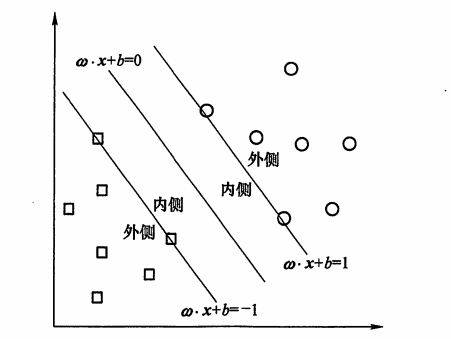
\includegraphics[width=0.45\textwidth]{pi/线性可分支持向量机.png} % 图片文件名和大小调整
  \caption{线性可分支持向量机示意图} % 图片的标题
  \label{fig:线性可分支持向量机} % 图片的标签,用于引用
\end{figure}
\begin{mydef}{普通支持向量}
定义9.2 式(9.1)中满足$(\omega\cdot a_i)+b=\pm1$成立的$a_i$称为普通支持向量。
\end{mydef}

对于线性可分的情况来说,只有普通支持向量在建立分类超平面的时候起到了作用, 它们通常只占样本集很小的一部分,故而也说明支持向量具有稀疏性。

对于$y_i=1$类的样本点,其与规范超平面的间隔为
$$\underset{y_{i}=1}{\operatorname*{min}}\frac{\mid(\omega\cdot a_{i})+b\mid}{\parallel\omega\parallel}=\frac{1}{\parallel\omega\parallel},$$
对于$y_{i}=-1$类的样本点,其与规范超平面的间隔为
$$\underset{y_{i}=-1}{\operatorname*{min}}\frac{\mid(\omega\cdot a_{i})+b\mid}{\parallel\omega\parallel}=\frac{1}{\parallel\omega\parallel},$$
则普通支持向量间的间隔为$\frac2{\|\omega\|}$。

最优超平面即意味着最大化$\frac2{\|\omega\|}$,$(\omega\cdot x)+b=\pm1$ 称为分类边界,于是
寻找最优超平面的问题可以转化为如下的二次规划问题,
$$\begin{array}{ll}\min&\frac{1}{2}\|\boldsymbol{\omega}\|^2,\\\mathrm{s.t.}&y_i[ (\boldsymbol{\omega}\cdot\boldsymbol{x}_i)+b ]\geqslant1 ,\quad i=1 ,\cdots,l.\end{array}
$$
\subsection{对偶问题}
该最优化的求解,除了一般的最优化算法,根据理论推导,有非常适用的SMO算法。

具体见\cite{周志华}$Page_{125}$  和\cite{司守奎}$Page_{251}$
\[
\begin{aligned}
& min_{\boldsymbol{\alpha}} \quad  \frac{1}{2} \sum_{i=1}^m \sum_{j=1}^m \alpha_i \alpha_j y_i y_j \boldsymbol{x}_i^\mathrm{T} \boldsymbol{x}_j-\sum_{i=1}^m \alpha_i\\
\text{s.t.} \quad & \sum_{i=1}^m \alpha_i y_i = 0 \\
& \alpha_i \geq 0, \quad i = 1, 2, \ldots, m
\end{aligned}
\]
\[\begin{aligned}\text{得到分类函数}\\&f(x)=\mathrm{sign}[\sum_{i=1}^{m}\alpha_{i}^{*}y_{i}(x_{i}\cdot x) +b^{*}] ,\end{aligned}
\]
\subsection{间隔的软化}
在前面的讨论中,我们一直假定训练样本在样本空间或特征空间中是线性可分的,即存在一个超平面能将不同类的样本完全划分开.然而,在现实任务中往往很难确定合适的核函数使得训练样本在特征空间中线性可分;退一步说, 即便恰好找到了某个核函数使训练集在特征空间中线性可分,也很难断定这个貌似线性可分的结果不是由于过拟合所造成的.

缓解该问题的一个办法是允许支持向量机在一些样本上出错.为此,要引入“软间隔”(soft margin)的概念


\begin{figure}[h!] % h! 表示“尽可能在当前位置插入”
  \centering % 图片居中
  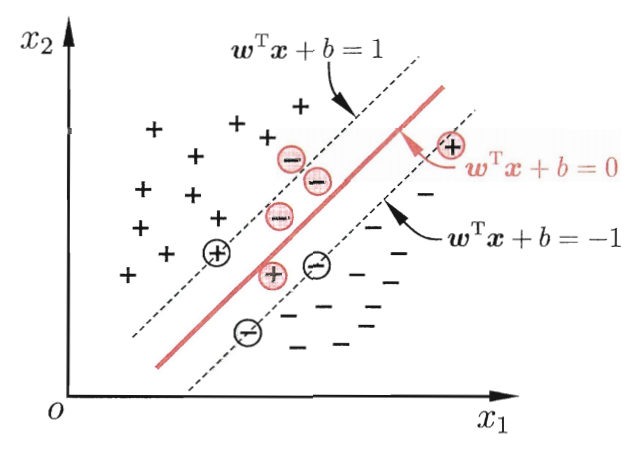
\includegraphics[width=0.45\textwidth]{pi/支持向量机的间隔软化.png} % 图片文件名和大小调整
  \caption{支持向量机的间隔软化示意图} % 图片的标题
  \label{fig:支持向量机的间隔软化} % 图片的标签,用于引用
\end{figure}


允许某些样本不满足约束

$y_i( \boldsymbol{w}^\mathrm{T} \boldsymbol{x}_i+ b) \geqslant 1$ .

当然,在最大化间隔的同时,不满足约束的样本应尽可能少.于是,优化目标可
写为
$$\min_{\boldsymbol{w},b}\:\frac{1}{2}\|\boldsymbol{w}\|^2+C\sum_{i=1}^m\ell_{0/1}\left(y_i\left(\boldsymbol{w}^\mathrm{T}\boldsymbol{x}_i+b\right)-1\right)\:,$$
其中$C>0$是一个常数,$\ell_{0/1}$是“0/1损失函数”
$$\ell_{0/1}(z)=\begin{cases}1,&\text{if }z<0;\\[2ex]0,&\text{otherwise}\end{cases}$$

然而,$\ell_0/1$ 非凸、非连续,数学性质不太好,使得式(6.29)不易直接求解.于是,人们通常用其他一些函数来代替$\ell_0/1$,称为“替代损失”(surrogate loss). 替代损失函数一般具有较好的数学性质,如它们通常是凸的连续函数且是$\ell_{0/1}$ 的上界. 图 6.5 给出了三种常用的替代损失函数:

hinge 损失:$\ell _{hinge}( z) = \max ( 0, 1- z)$ ;

指数损失(exponential loss$) : \ell _exp( z) = \exp ( - \dot{z} )$ ;

对率损失(logistic loss$) : \ell _log( z) = \log ( 1+ \exp ( - z) )$ .

引入“松弛变量” \(\xi_i \geq 0\),可以将支持向量机的优化问题重写为:

\[
\min_{\boldsymbol{w}, b, \boldsymbol{\xi}} \quad \frac{1}{2} \|\boldsymbol{w}\|^2 + C \sum_{i=1}^m \xi_i
\]

\[
\begin{aligned}
\text{s.t.} \quad & y_i (\boldsymbol{w}^\mathrm{T} \boldsymbol{x}_i + b) \geq 1 - \xi_i \\
& \xi_i \geq 0, \quad i = 1, 2, \ldots, m
\end{aligned}
\]

具体的推导见\cite{周志华}$Page_{131}$
\subsection{非线性模型与核函数}
暂时没写,见\cite{周志华}$Page_{126}$
\section{libsvm}
根据\cite{CC01a}
\href{https://www.csie.ntu.edu.tw/~cjlin/libsvm/}{https://www.csie.ntu.edu.tw/~cjlin/libsvm/}

该网站收录了libsvm的源码,可以下载下来阅读,也可以在github上搜索,在此将一些学习记录汇总在此,以便以后查阅。

\subsection{C-Support Vector Classification数学原理}
给定训练样本集$D=\{(\boldsymbol{x}_1,y_1),(\boldsymbol{x}_2,y_2),\ldots,(\boldsymbol{x}_l,y_l)\},y_i\in\{-1,+1\}$

求解如下优化问题
\begin{align*}
  \min_{w, b, \xi} \quad & \frac{1}{2} \|w\|^2 + C \sum_{i=1}^{l} \xi_i \\
  \text{s.t.} \quad & y_i (w \phi(x_i) + b) \geq 1 - \xi_i \quad \forall i = 1, \ldots, l \\
  & \xi_i \geq 0 \quad \forall i = 1, \ldots, l
  \end{align*}

  在这个优化问题中:
  \begin{itemize}
      \item \( w \) 是权重向量。
      \item \( b \) 是偏置项。
      \item \( \xi_i \) 是松弛变量。
      \item \( C \) 是惩罚参数,控制软间隔的宽度,C:C-SVC的惩罚参数,默认值为1.0,C越大, 相当于惩罚松弛变量,松弛变量越接近于0.趋向于数据集的全分对情况,但是其泛化能力减弱。相反,C越小,允许容错,将其当成噪声点,泛化能力变强。。
      \item \( \phi(x_i) \) 是特征映射函数,但我们通常使用函数$ K(x_i, x_j)= \phi(x_i)^T*\phi(x_j)$,即核函数。在本算法里面均是指RBF核$K(\mathbf{x}_{i},\mathbf{x}_{j})=\exp(-\gamma\|\mathbf{x}_{i}-\mathbf{x}_{j}\|^{2})$。
  \end{itemize}
根据KKT对偶条件(详情见\href{https://zhuanlan.zhihu.com/p/23549081}{https://zhuanlan.zhihu.com/p/23549081}和

\href{https://www.csie.ntu.edu.tw/~cjlin/papers/libsvm.pdf}{https://www.csie.ntu.edu.tw/~cjlin/papers/libsvm.pdf}),有

\begin{align*}
  &\min_{\alpha} \quad \frac{1}{2} \sum_{i=1}^{l} \sum_{j=1}^{l} \alpha_i \alpha_j y_i y_j K(x_i, x_j) - \sum_{i=1}^{l} \alpha_i \\
  \text{s.t.} \quad & 0 \leq \alpha_i \leq C \quad \forall i = 1, \ldots, l \\
  & \sum_{i=1}^{l} y_i \alpha_i = 0
\end{align*}

我们可以得到
\begin{equation}
  \begin{split}
      &\alpha_i = 0 \Rightarrow \beta_i = C \Rightarrow \xi_i = 0 \Rightarrow y_i (w \phi(x_i) + b) \geq 1 \\
      &0 < \alpha_i < C \Rightarrow 0 < \beta_i < C \Rightarrow \xi_i = 0 \Rightarrow y_i (w \phi(x_i) + b) = 1 \\
      &\alpha_i = C \Rightarrow \beta_i = 0 \Rightarrow \xi_i \geq 0 \Rightarrow y_i (w \phi(x_i) + b) \leq 1
  \end{split}
  \label{eq:支持向量判断公式}
  \end{equation}
也就是说我们可以根据$\alpha_i$的取值来判断该点$x_i$在什么位置
\subsubsection{SMO算法求解二次最优化问题}
\subsubsection{计算w和b}

假设我们已经得到了最优解$\{ \alpha^*_{i}, i = 1, \ldots, l \}$

根据式(\ref{eq:支持向量判断公式}),我们可以知道


$$w^*=\sum_{\alpha_{i}\neq 0}y_i\alpha_i^*\phi(x_i)$$

但我们这里并不需要显式地存储w,因为决策函数是

\begin{align*}sign(w^T\phi(x)+b)=&sign(\sum_{i=1}^ly_i\alpha_iK(x_i,x)+b)\\
  &=sign(\sum_{\alpha_{i}\neq 0}^ly_i\alpha_iK(x_i,x)+b)
\end{align*}

所以我们只需要储存支持向量($\alpha_i^* \neq 0$)对应的$\alpha_i^*y_i$和$b^*$即可

C-SVC和$\epsilon$-SVR中的b和one-class SVM中的$-\rho$是等价的,即$b=-\rho$,在LIBSVM中

存储的其实是$\rho$

根据式(\ref{eq:支持向量判断公式}),我们知道
$$b^*=y_i-\sum_{j=1}^ly_j\alpha_j^*K(x_j,x_i)$$

\subsection{参数寻优}
(惩罚参数$C$和RBF核的$\gamma$)







\section{2020-CUMCM-C}
\begin{myex}
  中小微企业的信贷决策
 
  在实际中,由于中小微企业规模相对较小,也缺少抵押资产,因此银行通常是依据信贷政策、企业的交易票据信息和上下游企业的影响力,向实力强、供求关系稳定的企业提供贷款,并可以对信誉高、信贷风险小的企业给予利率优惠。银行首先根据中小微企业的实力、信誉对其信贷风险做出评估,然后依据信贷风险等因素来确定是否放贷及贷款额度、利率和期限等信贷策略。
  某银行对确定要放贷企业的贷款额度为万元;年利率为0.04~0.15;贷款期限为1年。附件1\~3分别给出了123家有信贷记录企业的相关数据、302家无信贷记录企业的相关数据和贷款利率与客户流失率关系的2019年统计数据。该银行请你们团队根据实际和附件中的数据信息,通过建立数学模型研究对中小微企业的信贷策略,主要解决下列问题:
\begin{enumerate}
  \item 对附件1中123家企业的信贷风险进行量化分析,给出该银行在年度信贷总额固定时对这些企业的信贷策略。
  \item 在问题1的基础上,对附件2中302家企业的信贷风险进行量化分析,并给出该银行在年度信贷总额为1亿元时对这些企业的信贷策略。
  \item  企业的生产经营和经济效益可能会受到一些突发因素影响,而且突发因素往往对不同行业、不同类别的企业会有不同的影响。综合考虑附件2中各企业的信贷风险和可能的突发因素(例如:新冠病毒疫情)对各企业的影响,给出该银行在年度信贷总额为1亿元时的信贷调整策略。
\end{enumerate}
  附件1  123家有信贷记录企业的相关数据

  附件2  302家无信贷记录企业的相关数据

  附件3  银行贷款年利率与客户流失率关系的2019年统计数据
  
  附件中数据说明:

  (1) 进项发票:企业进货(购买产品)时销售方为其开具的发票。
  
  (2) 销项发票:企业销售产品时为购货方开具的发票。
  
  (3) 有效发票:为正常的交易活动开具的发票。
  
  (4) 作废发票:在为交易活动开具发票后,因故取消了该项交易,使发票作废。
  
  (5) 负数发票:在为交易活动开具发票后,企业已入账记税,之后购方因故发生退货并退款,此时,需开具的负数发票。
  
  (6) 信誉评级:银行内部根据企业的实际情况人工评定的,银行对信誉评级为D的企业原则上不予放贷。
  
  (7) 客户流失率:因为贷款利率等因素银行失去潜在客户的比率。
\end{myex}
问题的要点分析
\begin{itemize}
 \item 对于附件中的流水线数据,要学会统计数据的特征,查阅资料提取适当数量的指标或者属性
 \item 一般对于D级信誉的中小型企业不予发放贷款的信息,需要自己下来查询,数模比赛查资料的能力也是相当重要的。这样问题求解就会简便许多。
 \item 对于问题一确定了各中小型企业的各项指标之后,利用对有信誉记录的中小型企业的数据做多元回归分析或者机器学习,因变量是各违约风险,自变量是提取的各项指标。不同信誉评级下违约风险的描述性统计分析。
 常用的是将数据进行随机划分为训练集和测试集。 
 \item 对于问题二,将各种指标综合之后,对违约风险进行预测,或者是进行分类模型评价模型或者是得到信誉之后就能得出我们的信誉等级,剩下的可像问题一那样得出我们的违约风险。
 \item 搞定这几个模型就能进行多目标(如利润最高,风险和潜在损失最小)规划模型求解
 \item 对于问题三,可以考虑疫情影响继续构造指标,对结果进行划分,这个时候可将上市公司进行划分。
\end{itemize}

\section{2022-CUMCM-C}
\begin{myex}
  丝绸之路是古代中西方文化交流的通道,其中玻璃是早期贸易往来的宝贵物证。早期的玻璃在西亚和埃及地区常被制作成珠形饰品传入我国,我国古代玻璃吸收其技术后在本土就地取材制作,因此与外来的玻璃制品外观相似,但化学成分却不相同。
 
  玻璃的主要原料是石英砂,主要化学成分是二氧化硅$(SiO_2)$。由于纯石英砂的熔点较高, 为了降低熔化温度,在炼制时需要添加助熔剂。古代常用的助熔剂有草木灰、天然泡碱、硝石和铅矿石等,并添加石灰石作为稳定剂,石灰石煅烧以后转化为氧化钙$(CaO)$。添加的助熔剂不同,其主要化学成分也不同。例如,铅钡玻璃在烧制过程中加入铅矿石作为助熔剂,其氧化铅(PbO)、氧化钡(BaO)的含量较高,通常被认为是我国自己发明的玻璃品种,楚文化的玻璃就是以铅钡玻璃为主。钾玻璃是以含钾量高的物质如草木灰作为助熔剂烧制而成的,主要流行于我国岭南以及东南亚和印度等区域。
  
  古代玻璃极易受埋藏环境的影响而风化。在风化过程中,内部元素与环境元素进行大量交换,导致其成分比例发生变化,从而影响对其类别的正确判断。如图 1 的文物标记为表面无风化,表面能明显看出文物的颜色、纹饰,但不排除局部有较浅的风化;图 2 的文物标记为表面风化,表面大面积灰黄色区域为风化层,是明显风化区域,紫色部分是一般风化表面。在部分风化的文物中,其表面也有未风化的区域。

  现有一批我国古代玻璃制品的相关数据,考古工作者依据这些文物样品的化学成分和其他检测手段已将其分为高钾玻璃和铅钡玻璃两种类型。附件表单 1 给出了这些文物的分类信息, 附作表单 2 给出了相应的主要成分所占比例(空白处表示未检测到该成分)。这些数据的特点是成分性,即各成分比例的累加和应为 100%,但因检测手段等原因可能导致其成分比例的累加和非 100%的情况。本题中将成分比例累加利介于 85%-105%之间的数据视为有效数据。
  
  请你们团队依据附件中的相关数据进行分析建模,解决以下问题:
  
  问题 1 对这些玻璃文物的表面风化与其玻璃类型、纹饰和颜色的关系进行分析;皆合玻璃的类型,分析文物样品表面有无风化化学成分含量的统计规律,并根据风化点检测数据,预测其风化前的化学成分含量。
  分类结果的敏感性进行分析。
  
  问题 2 依据附件数据分析高钾玻璃、铅钡玻璃的分类规律;对于每个类别选择合适的化学成分对其进行亚类划分,给出具体的划分方法及划分结果,并对分类结果的合理性和敏感性进行分析。
  
  问题 3 对附件表单 3 中未知类别玻璃文物的化学成分进行分析,鉴别其所属类型,并对分类结果的合理性和敏感性进行分析
  
  问题 4 针对不同类别的玻璃文物样品,分析其化学成分之间的关联关系,并比较不同类
  别之间的化学成分关联关系的差异性。
\end{myex}

\begin{enumerate}

  \item 问题一:

数据预处理在这一问非常重要,颜色一列有缺失值,检测是否有异常值,成分之和在 85\%~105\%。

第一小问:要研究表面风化与玻璃类型、纹饰和颜色的关系, 这儿个变量都是离散值而非连续值,不适合米用皮尔逊相关系数,可以采用卡方检验的方式检测他们之间的相关性。分三组做卡方检验:表面风化-玻璃类型、表面风化-纹饰、表面风化-颜色。看网上还有别人用一些更高级的检验方式(fisher 检验、spearman 相关系数等等)。

第二小问:针对不同类型的玻璃,分析文物表面有无风化化学成分含量的统计规律,其实就是要看每一种成分在风化前和风华后含量的变化趋势,这里有一个问题,就是我们没有同一个文物上的同一种成分的变化趋势,不同文物上的成分含量是不能直接比较的,所以这里需要计算每种成分风化前后在各个文物中含量的统计量,来进行总体趋势的反馈。为了提高数据的维度,统计量应该包含一阶二阶统计量,如均值、方差、最值、中位数、峰度等等。有了这些统计量之后,就可以定性地说在风化前后这些统计量的变化怎么样。题目还要求我们定量分析,根据风化点检测数据,预测其风化前的化学成
 \item 问题二:

 第一小问要依据附件数据分析高钾玻璃、铅钡玻璃的分类规律,这就是要我们建立一个分类模型。常见的分类模型包括 SVM、决策树、随机森林、BP 神经网络等等,选择合适的模型,跑出结果,加以合理的解释即可。之后要我们对两类玻璃进行亚类划分,这其实就是要我们进行一个聚类。常见的聚类的方法有 Kmeans、层次聚类等等,按固定流程跑出结果并解释即可。这一问其实就是机器学习中有监督学习和无监督学习的应用。同时题目要求我们对结果进行合理性和敏感性分析,这就需要我们进行一些检验,如检测 SVM 分类的准确度、kmeans 中个体与中心的距离之和等等,以及做一些灵敏度检验。
\item 问题三:

这一问是对问题二的应用,问题二已经建立好了分类模型,将这个模型应用在问题三的分类上即可,把表单 3 中的数据输入到问题二的分类模型中,跑出结果并加以解释即可。

\item 问题四

针对不同类别的玻璃文物样品,要分析其化学成分之间的关联关系。计算变量之间的关联关系,可以采用相关系数、灰色关联分析、热力图等等。题目还要比较不同类别之间的化学成分关联关系的差异性,这里只需要把前面的关联模型在不同类别计算出的结果进行分析即可。



\end{enumerate}



\newpage
\bibliographystyle{plain} % 可以根据需要选择其他样式
\bibliography{modelref} % 你的bib文件名,不需要扩展名

\end{document}